\documentclass[11pt]{article}
\usepackage[a4paper,margin=1in]{geometry}
\usepackage{amsmath,amssymb}
\usepackage{tikz}
\usetikzlibrary{arrows.meta,positioning,calc}
\title{RAFAELIA QPU: Arquitetura Toroidal $\mathbb{T}^7$, Recorrência, Commit Gate e Programação Espectral}
\author{Projeto RAFAELIA}
\date{\today}
\begin{document}\maketitle
\begin{abstract}
Este whitepaper formaliza uma arquitetura quântica/neuromórfica virtual em $\mathbb{T}^7$ com 1000 osciladores, janela de 42 ciclos, commit gate com rollback, acoplamento fractal Mandelbrot e programação espectral.
\end{abstract}
\section{Modelo de Estado}
$\mathbf{s}=(u,v,\psi,\chi,\rho,\delta,\sigma)\in [0,1)^7$, $\mathbf{s}=\mathrm{ToroidalMap}(x)$, $x=(\text{dados},\text{entropia},\text{hash},\text{estado})$.
\section{Dinâmica}
\begin{align}
C_{t+1}&=(1-\alpha)C_t+\alpha C_{in},\; H_{t+1}=(1-\alpha)H_t+\alpha H_{in},\;\alpha=0.25\\
\phi&=(1-H)\cdot C,\quad F_{n+1}=F_n\frac{\sqrt3}{2}-\pi\sin(279^\circ),\quad x_{n+42}=x_n
\end{align}
\section{Pipeline de 42 ciclos}
\begin{center}
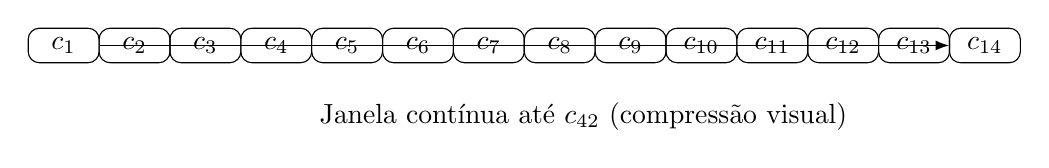
\begin{tikzpicture}[node distance=0.8cm,>=Latex]
\foreach \i in {1,...,14} {
  \node[draw,rounded corners,minimum width=0.9cm] (n\i) at (\i*0.9,0) {$c_{\i}$};
}
\draw[->] (n1)--(n14);
\node at (7.5,-0.9) {Janela contínua até $c_{42}$ (compressão visual)};
\end{tikzpicture}
\end{center}
\section{Rede de osciladores 10x10x10}
\begin{center}
\begin{tikzpicture}[scale=0.55]
\foreach \x in {0,...,9}
  \foreach \y in {0,...,9}
    \filldraw[blue!40] (\x,\y) circle (0.05);
\node at (4.5,-1) {Cada ponto representa uma coluna de 10 osciladores no eixo $z$};
\end{tikzpicture}
\end{center}
\section{Commit Gate e Rollback}
Ao final de cada janela, calcula-se paridade/integridade; se $\Pi<\Pi_{max}$, aplica-se rollback para checkpoint anterior.
\section{Acoplamento Fractal e Espectral}
$S(\omega)=\mathcal{F}[\Psi(t)]$, 
$R_L=\frac{\int S_L(\omega)H_{cardio}(\omega)d\omega}{\|S_L\|\|H_{cardio}\|}$,
$\mathcal{I}=\bigotimes_L (R_L\cdot\mathcal{F}(G_L))$.
\end{document}
